\documentclass{article}

% Language setting
% Replace `english' with e.g. `spanish' to change the document language
\usepackage[english]{babel}

% Set page size and margins
% Replace `letterpaper' with `a4paper' for UK/EU standard size
\usepackage[letterpaper,top=2cm,bottom=2cm,left=3cm,right=3cm,marginparwidth=1.75cm]{geometry}

% Useful packages
\usepackage{amsmath}
\usepackage{graphicx}
\usepackage[colorlinks=true, allcolors=blue]{hyperref}


% Packages for TODO List
\usepackage{enumitem,amssymb}
\newlist{todolist}{itemize}{2}
\setlist[todolist]{label=$\square$}
\usepackage{pifont}
\newcommand{\cmark}{\ding{51}}%
\newcommand{\xmark}{\ding{55}}%
\newcommand{\done}{\rlap{$\square$}{\raisebox{2pt}{\large\hspace{1pt}\cmark}}%
\hspace{-2.5pt}}
\newcommand{\wontfix}{\rlap{$\square$}{\large\hspace{1pt}\xmark}}

% Packages for glossaries
\usepackage[acronym]{glossaries}
\makeglossaries
\renewcommand{\glossarysection}[2][]{} % no title

% Package for booktabs table
\usepackage{booktabs}

% Packages and commands for Gantt chart
\usepackage{pgfgantt}
\usepackage{datetime} 
\usepackage{tikz}
\usepackage{pgfplots} % for tikz
\usetikzlibrary{shapes.geometric, arrows}
\def\checkmark{\tikz\fill[scale=0.4](0,.35) -- (.25,0) -- (1,.7) -- (.25,.15) -- cycle;} 

% Wrapfig for team contributions
\usepackage{wrapfig}
\usepackage{graphicx}

% ORCID: 
\usepackage{academicons}
\usepackage{tikz}
\usetikzlibrary{chains,positioning,shapes.symbols}
\usepackage{xcolor}
% \usepackage[final]{hyperref}
\definecolor{orcidlogocol}{HTML}{A6CE39}

\DeclareRobustCommand{\orcidicon}{%
	
\begin{tikzpicture}
	\draw[lime, fill=lime] (0,0) 
	circle [radius=0.16] 
	node[white] {{\fontfamily{qag}\selectfont \tiny ID}};
	\draw[white, fill=white] (-0.0625,0.095) 
	circle [radius=0.007];
	\end{tikzpicture}
	\hspace{-2mm}
}
\newcommand{\orcid}[1]{\href{https://orcid.org/#1}{\textcolor[HTML]{A6CE39}{\orcidicon}}}
% END ORCID

\usepackage{nicematrix} % for pugh chart

\usepackage{listings} % for code
\definecolor{codegreen}{rgb}{0,0.6,0}
\definecolor{codegray}{rgb}{0.5,0.5,0.5}
\definecolor{codepurple}{rgb}{0.58,0,0.82}
\definecolor{backcolour}{rgb}{0.95,0.95,0.92}

\lstdefinestyle{mystyle}{
    backgroundcolor=\color{backcolour},   
    commentstyle=\color{codegreen},
    keywordstyle=\color{magenta},
    numberstyle=\tiny\color{codegray},
    stringstyle=\color{codepurple},
    basicstyle=\ttfamily\footnotesize,
    breakatwhitespace=false,         
    breaklines=true,                 
    captionpos=b,                    
    keepspaces=true,                 
    numbers=left,                    
    numbersep=5pt,                  
    showspaces=false,                
    showstringspaces=false,
    showtabs=false,                  
    tabsize=2
}

\lstset{style=mystyle}

\title{EMAE 360 Report}
\author{You}

\begin{document}
\maketitle
\newpage

\tableofcontents
\newpage

\section*{Executive Summary}
\newpage

\section{Introduction}

Your introduction goes here! Simply start writing your document and use the Recompile button to view the updated PDF preview. Examples of commonly used commands and features are listed below, to help you get started.

Once you're familiar with the editor, you can find various project settings in the Overleaf menu, accessed via the button in the very top left of the editor. To view tutorials, user guides, and further documentation, please visit our \href{https://www.overleaf.com/learn}{help library}, or head to our plans page to \href{https://www.overleaf.com/user/subscription/plans}{choose your plan}.

\begin{figure}
    \centering
\begin{tikzpicture}
\begin{axis}[
    xlabel=Complexity of Document,
    ylabel=Time Spent Typesetting,
    legend pos=north west,
    xticklabels={\textit{Text Document}, \textit{Team Report}, \textit{Thesis}},
    xtick={1,2,3},
    yticklabels={,,},
    axis x line=bottom,
    axis y line=left,
    ]

    \addplot[color=red, mark=x] coordinates {
        (1, 1)
        (2, 3)
        (3, 6)
    };
    \addlegendentry{Word}

    \addplot[color=blue, mark=o] coordinates {
        (1, 2)
        (2, 2.5)
        (3, 3)
    };
    \addlegendentry{\LaTeX{}}

    \foreach \x in {1,2,3} {
        \draw[densely dotted] (\x,0) -- (\x,\pgfkeysvalueof{/pgfplots/ymax});
        \node[below, rotate=45, anchor=north east] at (\x,0) {\textit{\pgfkeysvalueof{/pgfplots/xticklabels}[\x]}};
    }
\end{axis}
\end{tikzpicture}


    \caption{Why you might want to use \LaTeX for this sort of project.}
    \label{fig:whylatex}
\end{figure}

\section{Goals and Objectives}

\newpage
\section{Scope}

\newpage
\section{Assigned and Derived Requirements}

\newpage
\section{System and Subsystem Design}
\textit{Repeat this section for different systems/subsystems.}

\subsection{Relevant Technical Information and Calculations}
\subsection{Drawings}
\textit{Include detail, assembly and CAD models!}
\subsection{Bill of Materials}
\textit{Consider using \url{www.tablesgenerator.com} to generate your table.}
\subsection{Materials and Manufacturing Methods}
\subsection{Quality Control/Critical Characteristics}

\newpage
\section{Assembly and Test}

\newpage
\subsection{Theory of Operations}

\newpage
\section{Failure Modes Effects Analysis (FMEA)}

\newpage
\section{Final Cost Estimate}

\newpage
\section{Design Satisfies Requirements}

\newpage
\section{Project Management}
\subsection{Task List}
\begin{itemize}
  \item Immediate plan of action.
  \begin{todolist}
  \item[\done] Frame the problem
  \item Write solution
  \item[\wontfix] profit
  \end{todolist}
\end{itemize}

\subsection{Gantt Chart}
\begin{ganttchart}[
vgrid,
x unit=.15cm,
y unit chart=.5cm,
time slot format=isodate,
today=2024-10-25,
today offset=.5,
today label=\today,
today label node/.append style=%
{anchor=north west},
today label font=\itshape\color{blue},
today rule/.style=%
{draw=blue, ultra thick}
]{2024-10-15}{2024-12-28}\\
\gantttitlecalendar{year, month=name}\\

\ganttmilestone{Meetings}{2024-11-2}
\ganttmilestone{}{2024-11-15}
\ganttmilestone{}{2024-11-30}
\ganttmilestone{}{2024-12-7}
\ganttmilestone{}{2024-01-11}
\ganttmilestone{}{2024-01-25}
\ganttmilestone{}{2024-02-08}
\ganttmilestone{}{2024-02-22}\\

\ganttbar[bar/.append style={fill=black}]{\checkmark Coauthor checklist}{2024-10-16}{2024-10-31} \\
\ganttbar[bar/.append style={fill=green}]{Abstract}{2024-10-30}{2024-11-3} \\
\ganttbar[bar/.append style={fill=}]{Plain Language Summary}{2024-10-25}{2024-11-1} \\

\ganttbar[progress=50, bar/.append style={fill=yellow}]{Tools}{2024-11-06}{2024-11-30} \\



\ganttbar[bar/.append style={fill=red}]{Holidays}{2024-12-05}{2024-1-5} \\


\ganttmilestone{Report}{2024-10-15}\\
\ganttmilestone{Goal for completing draft}{2024-12-25}\\

\end{ganttchart}

\newpage
\section{Team Contributions}

  \begin{wrapfigure}{l}{25mm} 
    
\includegraphics[width=1in,height=1.25in,clip,keepaspectratio]{figs/Vishner_N_20220311102144_443511.jpg}
  \end{wrapfigure}\par
  \textbf{Radar O'Reilly (Team Lead)\orcid{0000-0002-9846-8247}} is a fictional character in the M*A*S*H novels, film, the television series, the television pilot W*A*L*T*E*R and two episodes of the series After M*A*S*H. He was played by Gary Burghoff, and was one of only two actors to play a role in the 1970 film and then reprise their role for television; the other actor was G. Wood, who portrayed General Hammond, though he was just a recurring character in Season 1.\par \textit{Consider supplementing your summary with \url{https://www.elsevier.com/researcher/author/policies-and-guidelines/credit-author-statement}. Also, consider signing up for an ORCID at \url{orcid.org}.}


\newpage
\appendix

\newpage
\section{Team Charter}

\newpage
\section{Product Design Specification}
\textit{Given a set of numbers, there are elementary methods to compute its \acrlong{gcd}, which is abbreviated \acrshort{gcd}. 
This process is similar to that used for the \acrfull{lcm}. See Appendix \ref{sec:acronym} to understand why this paragraph is here... and then get rid of this paragraph.}


\newpage
\section{Pugh Charts}
\begin{table}[ht]
\centering
\caption{Pugh matrix}
\begin{NiceTabular}{lccc}[vlines]
\hline
\diagbox{Property}{Concept} & 
\RowStyle[cell-space-top-limit=3pt]{\rotate}
Concept 1 & Next concept & Next concept/increase line  \\
\hline
Do this                & $0$ & $0$  & $-$ \\
Do that                & $0$ & $0$  & $0$ \\
Do it quickly          & $0$ & $+$  & $+$ \\
Do the task quickly    & $0$ & $0$  & $-$ \\ 
\hline 
SUM:                   & $0$ & $+1$ & $+2$ \\
\hline
Ranking                & $2$ & $2$  & $1$  \\
\hline
Keep                   & NO  & NO   & YES \\
\hline
\end{NiceTabular}
\label{tab:Pugh_matrix2}
\end{table}

\section{Calculations}
\LaTeX{} is great at typesetting mathematics. Let $X_1, X_2, \ldots, X_n$ be a sequence of independent and identically distributed random variables with $\text{E}[X_i] = \mu$ and $\text{Var}[X_i] = \sigma^2 < \infty$, and let
\[S_n = \frac{X_1 + X_2 + \cdots + X_n}{n}
      = \frac{1}{n}\sum_{i}^{n} X_i\]
denote their mean. Then as $n$ approaches infinity, the random variables $\sqrt{n}(S_n - \mu)$ converge in distribution to a normal $\mathcal{N}(0, \sigma^2)$.

\section{List of Equations}
\textit{Note that you can reference an equation if you want to. Like this: Equation \ref{eqn:emc2}! Equation \ref{eqn:foo}! The numbering will automatically update.}

\begin{equation}
    \label{eqn:emc2}
    e = mc^2
\end{equation}

\begin{equation}
    \label{eqn:foo}
    x^n + y^n = z^n 
\end{equation}

\newpage
\section{List of Abbreviations}
\label{sec:acronym}
\newacronym{gcd}{GCD}{Greatest Common Divisor}
\newacronym{lcm}{LCM}{Least Common Multiple}
\newacronym{nasa}{NASA}{National Aeronautics and Space Administration}
\newacronym{lqtm}{LQTM}{Laughing Quietly To Myself}
\newacronym{wysiwyg}{WYSIWYG}{What You See Is What You Get}



\printglossary[type=\acronymtype]
\glsaddallunused[\acronymtype]

\newpage
\section{List of Symbols}
\begin{table}[h!]
\begin{tabular}{@{}llll@{}}
\toprule
Symbol & Meaning                            & Value & Unit \\ \midrule
$\pi$    & A geometric constant with no units and a nice long description& $\pi$   &      \\
$P$    & Power consumption                  &       & kW   \\
$L$    & Avogadro's number                  &   $6.02214076 \times 10^{23}$    & $mol^{-1}$   \\
$h$    & Height of tower                    &       & m    \\ \bottomrule
\end{tabular}
\end{table}

\newpage
\section{Some \LaTeX{} Examples and Tips}


\subsection{How to create Sections and Subsections}

Simply use the section and subsection commands, as in this example document! With Overleaf, all the formatting and numbering is handled automatically according to the template you've chosen. If you're using the Visual Editor, you can also create new section and subsections via the buttons in the editor toolbar.

\subsection{How to include Figures}

First you have to upload the image file from your computer using the upload link in the file-tree menu. Then use the includegraphics command to include it in your document. Use the figure environment and the caption command to add a number and a caption to your figure. See the code for Figure \ref{fig:frog} in this section for an example.

Note that your figure will automatically be placed in the most appropriate place for it, given the surrounding text and taking into account other figures or tables that may be close by. You can find out more about adding images to your documents in this help article on \href{https://www.overleaf.com/learn/how-to/Including_images_on_Overleaf}{including images on Overleaf}.

\begin{figure}
\centering
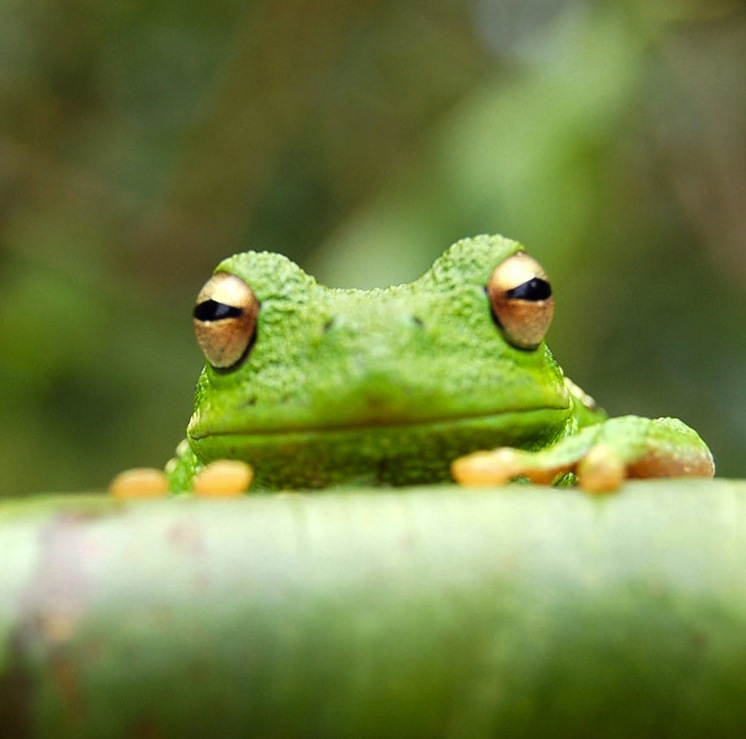
\includegraphics[width=0.25\linewidth]{frog.jpg}
\caption{\label{fig:frog}This frog was uploaded via the file-tree menu.}
\end{figure}

\subsection{How to add Tables}

Use the table and tabular environments for basic tables --- see Table~\ref{tab:widgets}, for example. For more information, please see this help article on \href{https://www.overleaf.com/learn/latex/tables}{tables}. 

\begin{table}
\centering
\begin{tabular}{l|r}
Item & Quantity \\\hline
Widgets & 42 \\
Gadgets & 13
\end{tabular}
\caption{\label{tab:widgets}An example table.}
\end{table}

\subsection{How to add Comments and Track Changes}

Comments can be added to your project by highlighting some text and clicking ``Add comment'' in the top right of the editor pane. To view existing comments, click on the Review menu in the toolbar above. To reply to a comment, click on the Reply button in the lower right corner of the comment. You can close the Review pane by clicking its name on the toolbar when you're done reviewing for the time being.

Track changes are available on all our \href{https://www.overleaf.com/user/subscription/plans}{premium plans}, and can be toggled on or off using the option at the top of the Review pane. Track changes allow you to keep track of every change made to the document, along with the person making the change. 

\subsection{How to add Lists}

You can make lists with automatic numbering \dots

\begin{enumerate}
\item Like this,
\item and like this.
\end{enumerate}
\dots or bullet points \dots
\begin{itemize}
\item Like this,
\item and like this.
\end{itemize}






\subsection{How to change the margins and paper size}

Usually the template you're using will have the page margins and paper size set correctly for that use-case. For example, if you're using a journal article template provided by the journal publisher, that template will be formatted according to their requirements. In these cases, it's best not to alter the margins directly.

If however you're using a more general template, such as this one, and would like to alter the margins, a common way to do so is via the geometry package. You can find the geometry package loaded in the preamble at the top of this example file, and if you'd like to learn more about how to adjust the settings, please visit this help article on \href{https://www.overleaf.com/learn/latex/page_size_and_margins}{page size and margins}.

\subsection{How to change the document language and spell check settings}

Overleaf supports many different languages, including multiple different languages within one document. 

To configure the document language, simply edit the option provided to the babel package in the preamble at the top of this example project. To learn more about the different options, please visit this help article on \href{https://www.overleaf.com/learn/latex/International_language_support}{international language support}.

To change the spell check language, simply open the Overleaf menu at the top left of the editor window, scroll down to the spell check setting, and adjust accordingly.

\subsection{How to add Citations and a References List}

You can simply upload a \verb|.bib| file containing your BibTeX entries, created with a tool such as JabRef. You can then cite entries from it, like this: \cite{greenwade93}. Just remember to specify a bibliography style, as well as the filename of the \verb|.bib|. You can find a \href{https://www.overleaf.com/help/97-how-to-include-a-bibliography-using-bibtex}{video tutorial here} to learn more about BibTeX.

If you have an \href{https://www.overleaf.com/user/subscription/plans}{upgraded account}, you can also import your Mendeley or Zotero library directly as a \verb|.bib| file, via the upload menu in the file-tree.

\subsection{Formatting code}
You have a couple of options for formatting code:
\begin{verbatim}
Text enclosed inside \texttt{verbatim} environment 
is printed directly 
and all \LaTeX{} commands are ignored.
\end{verbatim}

You can also use the \texttt{listings} package:
\begin{lstlisting}[language=Python, caption=Python example]
import numpy as np
    
def incmatrix(genl1,genl2):
    m = len(genl1)
    n = len(genl2)
    M = None #to become the incidence matrix
    VT = np.zeros((n*m,1), int)  #dummy variable
    
    #compute the bitwise xor matrix
    M1 = bitxormatrix(genl1)
    M2 = np.triu(bitxormatrix(genl2),1) 

    for i in range(m-1):
        for j in range(i+1, m):
            [r,c] = np.where(M2 == M1[i,j])
            for k in range(len(r)):
                VT[(i)*n + r[k]] = 1;
                VT[(i)*n + c[k]] = 1;
                VT[(j)*n + r[k]] = 1;
                VT[(j)*n + c[k]] = 1;
                
                if M is None:
                    M = np.copy(VT)
                else:
                    M = np.concatenate((M, VT), 1)
                
                VT = np.zeros((n*m,1), int)
    
    return M
\end{lstlisting}

See \url{https://www.overleaf.com/learn/latex/Code_listing} for further guidance.


\subsection{Using TikZ}
\label{sec:tikz}
You can use \href{https://texample.net//tikz/examples/}{TikZ} to create editable flowcharts and images that include cross-references. Note that this section is referenced in Figure \ref{fig:tikz1}. You can create tikz code in a \acrshort{wysiwyg} form on \url{mathcha.io}. Your computing language of choice may also have an option to export figures in tikz format. 

\begin{figure}
    \centering

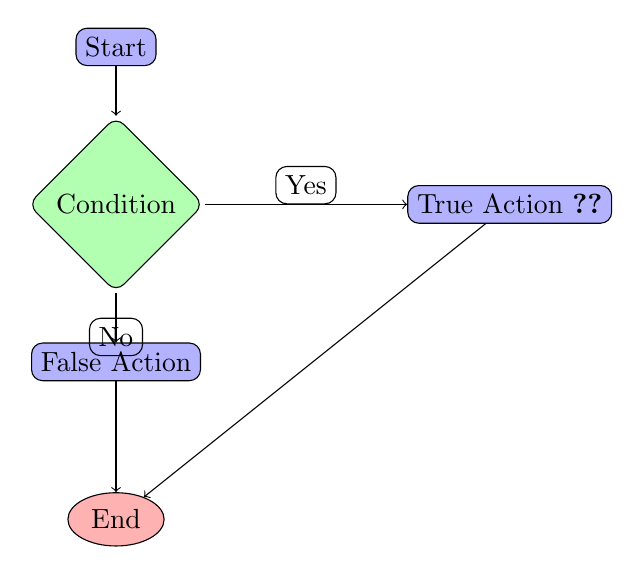
\begin{tikzpicture}[node distance=2cm,
    every node/.style={draw, rectangle, rounded corners, align=center},
    process/.style={fill=blue!30},
    decision/.style={diamond, fill=green!30},
    io/.style={trapezium, fill=yellow!30},
    terminal/.style={ellipse, fill=red!30}]

  \node[process] (start) {Start};
  \node[decision, below of=start] (dec1) {Condition};
  \node[process, right of=dec1, xshift=3cm] (true) {True Action \ref{sec:tikz}};
  \node[process, below of=dec1] (false) {False Action};
  \node[terminal, below of=false] (end) {End};

  \path[->] (start) edge (dec1);
  \path[->] (dec1) edge node[above] {Yes} (true);
  \path[->] (dec1) edge node[below] {No} (false);
  \path[->] (true) edge (end);
  \path[->] (false) edge (end);

\end{tikzpicture}

    \caption{Example TikZ figure. Code autogenerated by Google Gemini.}
    \label{fig:tikz1}
\end{figure}

\begin{figure}
    \centering
    % https://github.com/kwshi/pikachu-tikz/blob/master/pikachu-tikz.tex

\begin{tikzpicture}[x=.5in, y=.5in]
  \definecolor{deep green}{HTML}{346d33}
  \definecolor{light green}{HTML}{649935}
  \definecolor{bright green}{HTML}{6cad33}
  \definecolor{green}{HTML}{4e9429}
  \definecolor{cool green}{HTML}{2b5a3a}
  \definecolor{pale green}{HTML}{487e45}
  \definecolor{dark green}{HTML}{123214}
  \definecolor{sky}{HTML}{75c0a7}

  \definecolor{pants}{HTML}{934e33}
  \definecolor{pants stroke}{HTML}{443403}
  \definecolor{hand}{HTML}{ebb278}
  \definecolor{hand stroke}{HTML}{742f07}

  \definecolor{pikachu}{HTML}{efc41e}
  \definecolor{pikachu stroke}{HTML}{1f1f03}
  \definecolor{eartip}{HTML}{211e00}
  \definecolor{cheek}{HTML}{d05512}
  \definecolor{cheek stroke}{HTML}{993000}
  \definecolor{eye}{HTML}{510a01}
  \definecolor{glare}{HTML}{f4b97d}
  \definecolor{nose}{HTML}{692601}
  \definecolor{mouth}{HTML}{711900}
  \definecolor{tongue}{HTML}{ea8159}

  \tikzset{
    stroke/.style={line width=.6ex, draw=#1},
    eye/.pic={
      \draw [stroke=eye, fill=eye]
      (0,0)
      .. controls +(-.1,-.1) and +(-.2,0) .. (.2,-.4)
      .. controls +(.2,0) and +(0,-.2) .. (.4,-.2)
      .. controls +(0,.3) and +(.1,.1) .. cycle;
      \fill [glare, path fading={
        circle with fuzzy edge 20 percent
      }]
      (.1,-.1) circle [radius=.1];
    },
  }

  \clip [rounded corners=1ex, preaction={fill=sky}]
  (0,0) rectangle (7,6);

  \fill [light green]
  (4,7) -- (4.9,4)
  .. controls (5,5.8) and (5.4,5.9) .. (7,5.8)
  |- (0,0) |- cycle;

  \fill [bright green]
  (5.4,5)
  .. controls (5.5,4.8) and (6.7,4.8) .. (6.8,4.9)
  .. controls (6.9,5) and (6.7,5.4) .. (6.5,5.5)
  .. controls (6.3,5.6) and +(.2,.1) .. (5.7,5.5)
  .. controls +(-.2,-.1) and (5.3,5.1) .. cycle

  (1.2,5.5)
  .. controls (1.5,5.2) and (1.7,5.3) .. (1.1,7)
  -- cycle;

  \fill [deep green]
  (7,4) -- (4,3) -- (2.2,4.9)
  .. controls +(-.2,0) and +(.2,.2) .. (1.4,4.5)
  -- (1.7,3.7)
  .. controls +(-.2,-.3) and +(.7,.3) .. (.7,3.9)
  -| (0,0) -| cycle;

  \fill [cool green]
  (2.2,3.3)
  .. controls +(-.1,-.1) and +(.1,0) .. (1.8,3.1)
  .. controls +(-.2,0) and +(.3,0) .. (1,3.3)
  .. controls +(-.3,0) and +(.3,-.2) .. (.3,2.9)
  -- (0,1.7)
  .. controls +(.2,-.2) .. (5,2)

  (7,4) -- (4,3) -- (6,2.6)
  .. controls +(.3,.4) and +(-.3,-.2) .. (7,2.8);

  \fill [dark green]
  (.3,1.7)
  .. controls +(0,-.2) and +(-.3,0) .. +(.5,-.3)
  .. controls +(.3,0) and +(0,-.2) .. +(1.1,-.1)
  .. controls +(0,.3) and +(.4,0) .. +(.5,.4)
  .. controls +(-.3,0) and +(0,.2) .. cycle

  (1.9,2.9)
  .. controls +(-.1,0) and +(.1,.2) .. +(-.3,-.3)
  .. controls +(-.1,-.2) and +(-.2,0) .. +(-.1,-.5)
  .. controls +(.1,0) and +(-.1,-.2) .. +(.2,-.3)
  .. controls +(.1,.2) and +(.3,0) .. cycle;

  \fill [pale green]
  (2.2,2.4)
  .. controls +(-.8,.3) and +(.8,0) .. (.9,1.4)
  .. controls +(-.3,0) and +(-.3,0) .. (.7,1.3)
  .. controls +(.9,0) and +(-1.6,0) .. (2.1,1);

  \fill [green]
  (7,2.5)
  .. controls +(-.6,-.1) and +(.1,.7) .. (6.2,1.7)
  .. controls +(0,-.5) and +(-.2,0) .. (7,1.3)

  (2.2,.6)
  .. controls +(-1.5,.2) and +(.4,-.2) .. (.6,.7)
  .. controls +(-.2,.1) and +(.2,.1) .. (0,.7)
  -- (0,.6)
  .. controls +(.7,.1) and +(-.7,0) .. (.8,.3)
  .. controls +(.4,0) and +(.1,.2) .. (1.2,0)
  -- (3,0) |- (2.4,.3)
  -- (2.3,.5)

  (7,1)
  .. controls +(-.2,0) and +(.2,.2) .. (6.4,.7)
  .. controls +(.2,-.1) and +(-.2,0) .. (7,.6);


  \fill [pants, stroke=pants stroke]
  (-.1,1)
  .. controls (0,2) and (1,5) .. (1.6,6.4)
  .. controls (2.4,5) and (2.8,1) .. (3.2,0)
  -- (6,0)
  .. controls (4.6,6) .. (4.4,6.6)
  -- (-2,8) -- cycle;

  \fill [hand, stroke=hand stroke]
  (-.1,5.5)
  .. controls (.5,5.6) and (.8,5.8) .. (.9,7)
  -- (-1,8) -- cycle;

  \newcommand{\pikachu}{
    (6.7,-.1)
    .. controls (6.6,.8) and (6.4,1.3) .. (6.2,1.9)
    .. controls (6,2.5) and (6,2.6) .. (5.8,3)
    -- +(.1,-.1)
    .. controls (6.6,3.4) and (7.2,4) .. (8,4.8)
    .. controls (7,4.6) and (5.8,4) .. (5.4,3.8)
    .. controls (5.2,3.7) and (5,3.7) .. (5,3.7)
    .. controls (4.4,3.7) and (4.2,3.7) .. (3.2,3.6)
    .. controls (1.8,4.6) and (1.2,4.8) .. (.9,5)
    .. controls +(.6,-1) and +(-.8,.7) .. (2.4,3)
    -- +(.1,.1)
    .. controls +(-.3,-.5) and (2.2,2.2) .. (2.1,1.7)
    .. controls (2,1.3) and (2,1.1) .. (2,1)
    .. controls (2,.7) and (2.4,.4) .. (2.4,.2)
    .. controls (2.4,0) and (2.2,-.2) .. (2.2,-.4)
    -- (4,-1) -- cycle
  }
  \begin{scope}
    \clip [preaction={fill=pikachu}] \pikachu;

    \fill [eartip]
    (1.8,3.5)
    .. controls (1.2,4.6) and +(-.1,-.1) .. (1.5,4.7)
    -- (0,6) -- cycle;

    \pic [at={(2.8,2.4)}] {eye};
    \pic [at={(4.7,2.4)}] {eye};

    \draw [stroke=nose, fill=nose] (3.6,1.8)
    .. controls +(-.1,0) and +(-.2,0) .. +(.2,-.1)
    .. controls +(.1,0) and +(.3,0) .. cycle;

    \draw [stroke=cheek stroke, fill=cheek]
    (2,1.2)
    .. controls +(0,-.1) and +(-.2,0) .. +(.4,-.3)
    .. controls +(.2,0) and +(0,-.3) .. +(.7,.1)
    .. controls +(0,.2) and +(.2,0) .. +(.3,.4)
    .. controls +(-.2,0) and +(0,.3) .. cycle

    (5.2,1.3)
    .. controls +(0,-.2) and +(-.2,0) .. +(.3,-.4)
    -- +(.4,-.4)
    .. controls +(.2,0) and +(0,-.3) .. +(.7,0)
    .. controls +(0,.1) and +(.2,0) .. +(.4,.3)
    -- +(.3,.3)
    .. controls +(-.2,0) and +(0,.1) .. cycle;

    \newcommand{\mouth}{
      (3.5,1.2)
      .. controls +(-.1,-.1) and +(-.1,.2) .. +(0,-.4)
      .. controls +(.1,-.2) and +(-.1,0) .. +(.4,-.6)
      .. controls +(.1,0) and +(-.1,-.1) .. +(.7,-.5)
      .. controls +(.1,.1) and +(.1,-.1) .. +(.7,0)
      .. controls +(-.1,.1) and +(.1,.1) .. cycle
    }
    \begin{scope}
      \clip [postaction={fill=mouth}] \mouth;

      \fill [tongue]
      (4,1.3)
      .. controls +(-.2,-.1) and +(0,.4) .. (3.5,.8)
      -- ++(0,-1) -| +(2,2) -- cycle;
    \end{scope}
    \draw [stroke, draw=mouth] \mouth;
  \end{scope}
  \draw [stroke, draw=eartip] \pikachu;
\end{tikzpicture}
    \caption{Unwieldy code? You can \texttt{$\backslash$include} it in a separate file. }
    \label{fig:tikz2}
\end{figure}

\subsection{Pandoc}
If you already have code in Markdown or another format, consider using \href{https://pandoc.org/demos.html}{pandoc} to convert it. Very useful!



\subsection{Good luck!}

We hope you find Overleaf useful, and do take a look at our \href{https://www.overleaf.com/learn}{help library} for more tutorials and user guides! Please also let us know if you have any feedback using the Contact Us link at the bottom of the Overleaf menu --- or use the contact form at \url{https://www.overleaf.com/contact}.

\bibliographystyle{alpha}
\bibliography{sample}

\end{document}